\providecommand{\Bezier}{B\'{e}zier}
\providecommand{\bezier}{b\'{e}zier}

\title{Calculus II Applications to \Bezier\ Curves: Normal, Tangent, and Bounds}
\author{Jeff W McGlynn}
\date{\today}

\documentclass[oneside,usepdftitle=true]{article}
\usepackage{color} %used for font color
\usepackage{amssymb} %maths
\usepackage{amsmath} %maths
\usepackage[utf8]{inputenc} %useful to type directly diacritic characters
\usepackage{graphicx}
\usepackage{subfigure}
\usepackage[pdfusetitle,bookmarksnumbered,plainpages=false]{hyperref} % For synchronizing author and title with the PDF.

% Set up margins.
\usepackage[margin=1in]{geometry} % Set up margins.

\hypersetup{pdfborder=0 0 0}

% Set up helper commands.
\providecommand{\norm}[1]{\lVert#1\rVert}

\begin{document}
\maketitle
\tableofcontents
\setcounter{tocdepth}{2}

\newpage

\section{Derivative}
\label{sec:Derivative}

\subsection{General Equation}
The general equation for a \Bezier\ curve is:

\begin{equation}\label{eqn:bezier_general}
	\mathbf{B}(t) = \sum_{i=0}^n {n\choose i} (1 - t)^{n - i} t^i \mathbf{P}_i
\end{equation}

Since we are taking the derivative with respect to $t$, only the Bernstein polynomial effects the derivative.  The Bernstein polynomial is:

\[ B_{n,i}(t) = {n\choose i} (1 - t)^{n - i} t^i \]

Or, expanded:

\[ B_{n,i}(t) = \cfrac{n!}{i! (n - i)!} (1 - t)^{n - i} t^i \]

\subsection{Finding the Bernstein Polynomial's Derivative}

The derivative of this is:

\[ B_{n,i}'(t) = \cfrac{n!}{i! (n - i)!} [ it^{i - 1} (1 - t)^{n - i}] - \cfrac{n!}{i! (n - i)!}[t^i (n - i)(1 - t)^{n - i - 1}] \]

By simplifying and pulling out an $n$, this simplifies to:

\[ B_{n,i}'(t) = n \cfrac{(n - 1)!}{(i - 1)! (n - i)!} [ t^{i - 1} (1 - t)^{n - i}] - n \cfrac{(n - 1)!}{i! (n - i - 1)!}[t^i (1 - t)^{n - i - 1}] \]

Observe that this equation is now composed of two different Bernstein polynomials.  After substituting them in, the equation becomes:

\begin{equation}\label{eqn:bernstein_deriv}
	B_{n,i}'(t) = n [ B_{n-1,i-1}(t) - B_{n-1,i}(t) ]
\end{equation}

The derivative of the internal Bernstein polynomial is now known.  It is substituted back into the general equation for a \Bezier\ curve:

\begin{eqnarray}
	\nonumber \mathbf{B}'(t) &=& \sum_{i=1}^{n} B_{n,i}'(t) \mathbf{P}_i \\
	\nonumber \mathbf{B}'(t) &=& n \sum_{i=1}^{n} [ B_{n-1,i-1}(t) - B_{n-1,i}(t) ] \mathbf{P}_i \\
	\label{eqn:bezier_der_close}
	\mathbf{B}'(t) &=& n \sum_{i=0}^{n-1} [ B_{n-1,i}(t) - B_{n-1,i+1}(t) ] \mathbf{P}_{i+1}
\end{eqnarray}

Note the interference pattern that is created by subtracting $B_{n,i+1}$ in Equation \eqref{eqn:bezier_der_close}{.}  Using this, the derivative of \eqref{eqn:bezier_general} can be rewritten as:

\subsection{General Derivative}\label{sec:gen_deriv}

\begin{equation}\label{eqn:bezier_deriv}
	\mathbf{B}'(t) = n \sum_{i=0}^{n-1} B_{n-1,i}(t) [ \mathbf{P}_{i+1} - \mathbf{P}_i ]
\end{equation}

This is the general derivative of a \Bezier\ curve.




\section{Tangent Vector}

\begin{figure}[htp]
\begin{center}
	
	\subfigure[Cubic \Bezier\ Curve]{
		\label{fig:bezier_spline}
		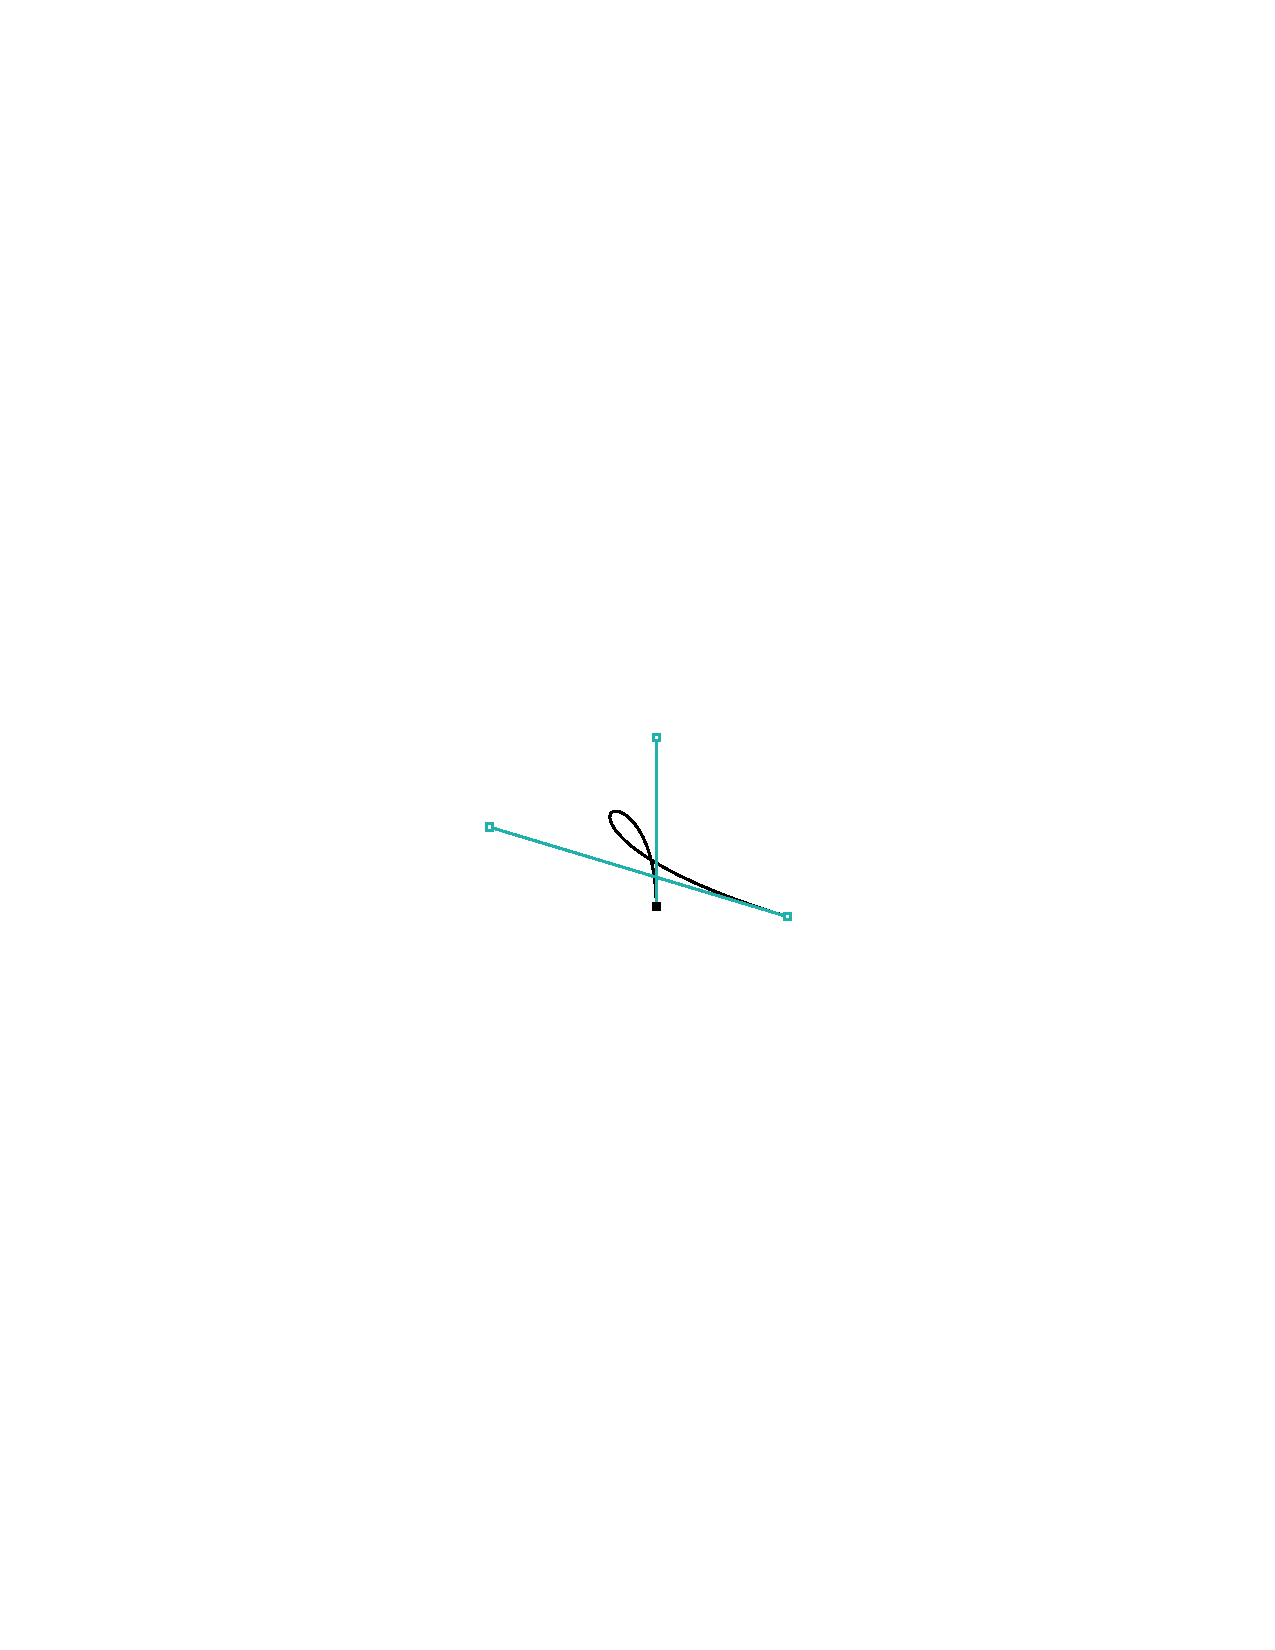
\includegraphics{figure_bezier_spline}
	}
	\subfigure[Derivative of \ref{fig:bezier_spline}]{
		\label{fig:bezier_spline_deriv}
		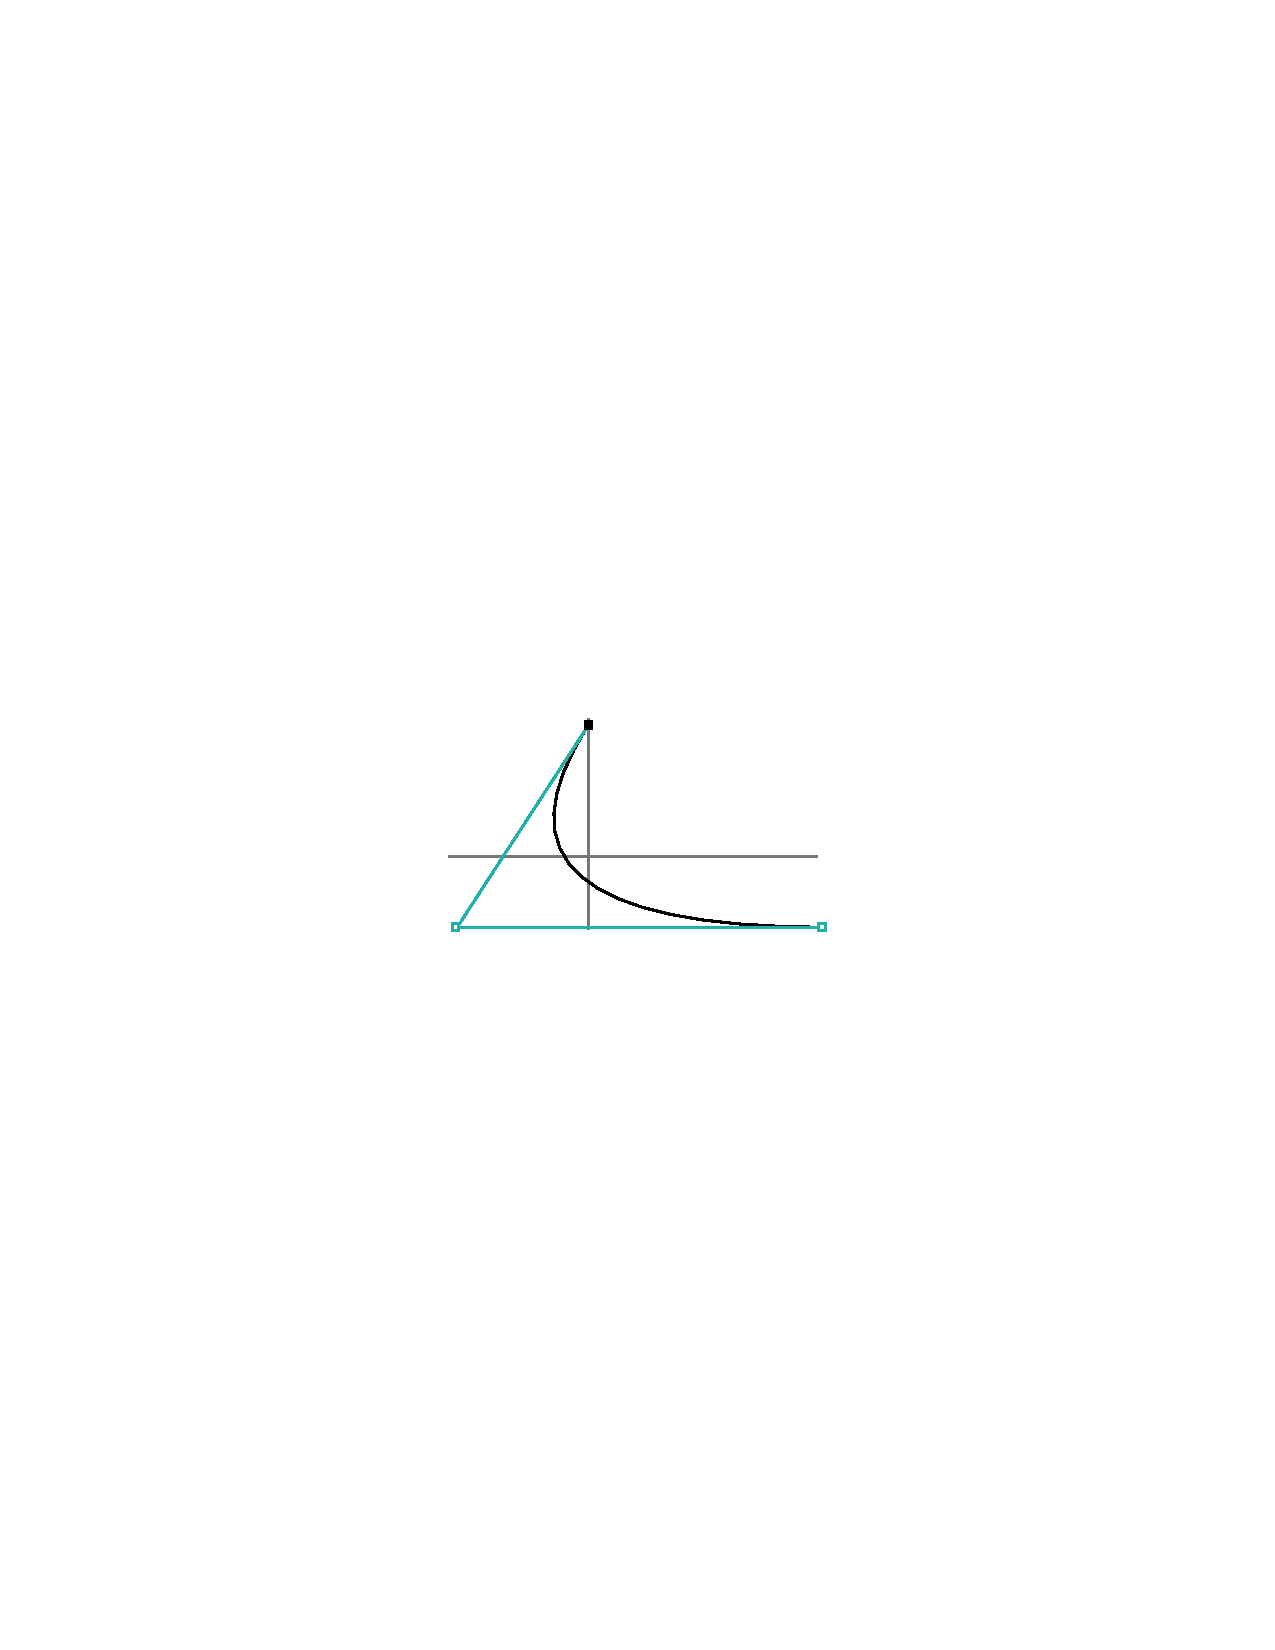
\includegraphics{figure_bezier_spline_deriv}
	}
	
	\caption{Cubic \Bezier\ Curve and Derivative}
\end{center}
\end{figure}

As $\mathbf{B}(t)$ is a vector, the normalized first derivative is the direction of the tangent vector, or $\mathbf{N}(t).$

\begin{equation}\label{eqn:bezier_tangent}
	\mathbf{N}(t) = \cfrac{\sum_{i=0}^{n-1} n B_{n-1,i}(t) [ \mathbf{P}_{i+1} - \mathbf{P}_i ]}{\norm{\sum_{i=0}^{n-1} n B_{n-1,i}(t) [ \mathbf{P}_{i+1} - \mathbf{P}_i ]}}
\end{equation}



\section{Normal Vector}

The normal vector is the normalized second derivative of the \Bezier\ curve equation \eqref{eqn:bezier_general}.

\subsection{Bernstein Polynomial}
First, we find the second derivative of the Bernstein polynomial \eqref{eqn:bernstein_deriv}.

\begin{eqnarray}
	\nonumber B_{n,i}'(t) &=& n [ B_{n-1,i-1}(t) - B_{n-1,i}(t) ] \\
	\nonumber B_{n,i}''(t) &=& n[ B_{n-1,i-1}'(t) - B_{n-1,i}'(t) ] \\
	\nonumber B_{n,i}''(t) &=&  n[(n-1)[B_{n-2,i-2} - B_{n-2,i-1}] - (n-1)[B_{n-2,i-1} - B_{n-2,i}]] \\
	\label{eqn:bernstein_second_deriv}
	B_{n,i}''(t) &=& n (n-1) [B_{n-2,i-2} - 2 B_{n-2,i-1} + B_{n-2,i}]
\end{eqnarray}

\subsection{General Equation}

Now, the second derivative of the Bernstein polynomial is used to find the second derivative of the general equation:

\begin{eqnarray}
	\nonumber \mathbf{B}''(t) &=& n (n-1) \sum_{i=2}^n [B_{n-2,i-2} - 2 B_{n-2,i-1} + B_{n-2,i}] \mathbf{P}_i \\
	\label{eqn:bezier_second_der_close}
	\mathbf{B}''(t) &=& n (n-1) \sum_{i=0}^{n-2} [B_{n-2,i} - 2 B_{n-2,i+1} + B_{n-2,i+2}] \mathbf{P}_{i+2}
\end{eqnarray}

By using the same logic used to derive the general \Bezier\ derivative in section \ref{sec:gen_deriv}, the general equation of the second derivative reduces to:

\begin{equation}\label{eqn:bezier_second_deriv}
	\mathbf{B}''(t) = n (n - 1) \sum_{i=0}^{n-2} B_{n-2,i}(t) [ \mathbf{P}_{i+2} - 2\mathbf{P}_{i+1} + \mathbf{P}_i ]
\end{equation}





\section{Computing Bounds}

The bounds of a \Bezier\ curve coincide with its extrema.  To find the extrema, use the first derivative test to find critical points.

Critical points are found by setting $\mathbf{B}'(t) = 0$ and solving for $t$.  To confirm, the second derivative test may be used, but it is often computationally faster to consider all critical points when determining the bounding box instead of classifying them.

For a cubic curve, the derivative is a quadratic curve which can be solved with the quadratic equation.

% Print the bibliography.
\newpage
\nocite{cs-lecture,bez-paper} % Automatically use cs-lecture and bez-paper, even if they aren't cited.

\bibliographystyle{plain}
\bibliography{citations}

\end{document}
